\documentclass{article}

% pacakages
\usepackage[french]{babel}
\usepackage{caption}
\usepackage[T1]{fontenc}
\usepackage{amsmath, amsfonts, amssymb}
\usepackage{stmaryrd}
\usepackage{fancyhdr}
\usepackage{lastpage}
\usepackage{lipsum}
\usepackage{cprotect}
\usepackage{graphicx}
\usepackage[ddmmyyyy]{datetime}
\usepackage{adjustbox}
\usepackage[a4paper, portrait, margin=20mm]{geometry} % define the page format
\usepackage[explicit]{titlesec}
\usepackage{color, soul}
\setulcolor{red}

%reference for the items of 'enumerate'
\usepackage{enumitem, hyperref}
\makeatletter
\def\namedlabel#1#2{\begingroup
    #2%
    \def\@currentlabel{#2}%
    \phantomsection\label{#1}\endgroup
}
\makeatother

%enumerate style
\renewcommand{\labelenumi}{\arabic{enumi}.}

%personalized section style
\titleformat{\section}
{\Large\bfseries}
{\thesection}{1em}{\ul{#1}}

%code formatting
\usepackage{minted}
\usemintedstyle{manni}

%divers commands
\newcommand{\bb}[1]{\mathbb{#1}}
\newcommand{\encadrer}[1]{\fbox{color=red
    \begin{minipage}{0.90\textwidth}
        #1
    \end{minipage}
}}
% \renewcommand{\thesection}{\Roman{section}} % Roman numerals for sections
\setlength{\headheight}{12.5pt}

\graphicspath{ {./img/} } % define path to img 
\newcommand{\image}[3]{ %command to insert image
    \begin{minipage}[t]{\linewidth}
        #1
        \adjustbox{valign=t}{
            \includegraphics[width=#2\linewidth]{#3}
        }
    \end{minipage}}

%page numerotation
\pagestyle{fancy}
\fancyhf{}
\renewcommand{\headrulewidth}{0pt}
\fancyfoot[R]{\thepage/\pageref{LastPage}}

%document info
\makeatletter
\title{DM2 - Mines MP 2019}
\date{\today}
\newcommand{\matiere}{Informatique Option}
\newcommand{\classe}{MP\textsuperscript{*} }
\author{Arsène MALLET}

%header
\fancypagestyle{firstpage}{
    \fancyhead[L]{\@author}
    \fancyhead[C]{\classe - \matiere}
    \fancyhead[R]{\@date}
}


\begin{document}

\thispagestyle{firstpage}

\begin{center}
    \huge\bfseries{\@title}
\end{center}

\section{Premiers exemples}

\begin{enumerate}
    \item Le langage reconnu par l'automate $A_1$ est l'ensemble des \fbox{mots de taille impaire}.
    \item Le langage reconnu par l'automate $A_2$ est l'ensembles des \fbox{mots contenant un nombre impair de $b$}.
    \item $\boxed{L(A_1) = (a \cdot a|b \cdot b|a \cdot b|b \cdot a)^* \cdot (a|b)}$
    \item $\boxed{L(A_1) = (a|b \cdot a^* \cdot b)^*\cdot b\cdot a^*}$
    \item \begin{minted}{ocaml}
    let a2 = 2, [|0, 1 ; 1, 0|], [|false; true|]  ;;
    \end{minted}
\end{enumerate}

\section{\'Etats accessibles d'un automate}

\begin{enumerate}
    \setcounter{enumi}{5}

    \item \begin{minted}{ocaml}
    let numero n a =
        let t = Array.make n (-1) in
        let rec aux index = function (*parcours la liste*)
          |[] -> ()
          |h::q -> t.(h) <- index ; aux (index + 1) q in
        aux 0 a ; t ;;
    \end{minted}

    \item \begin{minted}{ocaml}
    let etats_accessibles aut = 
        let n, delta, f = aut in 
        let visited = Array.make n false in
        let parcours = ref [] in
        let aux etat =
            if not visited.(etat) then 
                begin
                visited.(etat) <- true ;
                parcours := etat :: !parcours ;
                let succ_a, succ_b = delta.(etat) in
                aux succ_a ;
                aux succ_b
                end in 
        aux 0 ;;
        List.rev !parcours
    \end{minted}
    \underline{Compl\'exit\'e} : La création d'une \verb|Array| de taille $n$ est en $O(n)$, et l'accés à un élément d'une liste, tout comme la concatenation d'un élément avec une liste, sont en $O(1)$. On ne s'intéresse donc qu'aux appels récursifs de la fonction \verb|aux|. Comme $|Q| = n$, et que pour tout $q \in Q$, il existe deux \'etats $q_1$ et $q_2$ (potentiellement égaux) tels que $\delta(q, a) = q_1$ et $\delta(q, b) = q_2$, la fonction \verb|aux| fait au plus $2^n$ appels récursifs, soit une compléxité en $\boxed{O(2^n)}$.

    \item \begin{minted}{ocaml}
    let partie_accessible aut = 
        let n, delta, f = aut in
        let new_etats = etats_accessibles aut in 
        let apparition = numero n new_etats in
        let new_n = List.length new_etats in
        let new_delta = Array.make new_n (0,0) in
        let new_f = Array.make new_n false in
        let rec aux = function
            |[] -> (new_n, new_delta, new_f)
            |h::t -> let s = apparition.(h) in
                    new_f.(s) <- f.(h);
                    let succ_a, succ_b = delta.(h) in
                    new_delta.(s) <- apparition.(succ_a) ,apparition.(succ_b);
                    aux t in
        aux new_etats ;;
    \end{minted}

\end{enumerate}

\section{Morphismes d'automates}

\subsection{Exemples de morphismes d'automates}

\begin{enumerate}
    \setcounter{enumi}{8}

    \item $\varphi : \mathcal{A}_3 \rightarrow \mathcal{A}_2$ est représentée par \begin{tabular}{|c|c|}
        \hline
        $q$ & $\varphi(q)$ \\
        \hline
        $E$ & $C$ \\
        \hline
        $F$ & $C$ \\
        \hline
        $G$ & $D$ \\
        \hline
    \end{tabular}

    \item $\varphi : \mathcal{A}_4 \rightarrow \mathcal{A}_2$ est représentée par \begin{tabular}{|c|c|}
        \hline
        $q$ & $\varphi(q)$ \\
        \hline
        $H$ & $C$ \\
        \hline
        $I$ & $C$ \\
        \hline
        $J$ & $D$ \\
        \hline
        $K$ & $D$ \\
        \hline
    \end{tabular}

    \item Supposons qu'il existe un morphisme d'automate $\varphi  : \mathcal{A}_1 \rightarrow \mathcal{A}_2$, alors, pour vérifier $(2)$ : $\varphi(A) = B$, et pour vérifier $(4)$ : $\varphi(B) = D$. Or si $\varphi$ est un morphisme d'automates, alors d'après $(3)$,
    \begin{eqnarray*}
        \varphi(\delta_{\mathcal{A}_1}(A, a)) & = & \varphi(B) \\
        & = & D \\
        & = & \delta_{\mathcal{A}_2}(\varphi(A), a)
    \end{eqnarray*}
    Mais, $\varphi(A) = C$ d'après $(1)$, donc 
    \begin{eqnarray*}
        \delta_{\mathcal{A}_2}(\varphi(A), a) & = & \delta_{\mathcal{A}_2}(C, a) \\
        & = & D \\
        & = & C \\ 
        & \rightarrow & \text{\underline{Absurde !}}
    \end{eqnarray*}
    Ainsi, \fbox{il n'existe pas de morphisme d'automates de $\mathcal{A}_1$ vers $\mathcal{A}_2$}.

    \item Comme à la question précédente, supposons qu'il existe un morphisme d'automate $\varphi  : \mathcal{A}_5 \rightarrow \mathcal{A}_2$, alors $(2)$ et $(4)$ nous donne : $\varphi(L) = C$, $\varphi(M) = D$ et $\varphi(N) = C$ (car $N \notin F_{\mathcal{A}_5}$). $(3)$ impose alors, 
    \begin{eqnarray*}
        \varphi(\delta_{\mathcal{A}_5}(N, b)) & = & \varphi(L) \\
        & = & C \\
        & = & \delta_{\mathcal{A}_2}(\varphi(N), b) \\
        & = & \delta_{\mathcal{A}_2}(C, b) \hspace{5mm} (\varphi(N) = C) \\
        & = & D \\
        & \rightarrow & \text{\underline{Absurde !}}
    \end{eqnarray*}
    Ainsi, \fbox{il n'existe pas de morphisme d'automates de $\mathcal{A}_5$ vers $\mathcal{A}_2$}.

\end{enumerate}

\subsection{Propri\'et\'es des morphismes d'automates}

\begin{enumerate}
    \setcounter{enumi}{12}

    \item \label{itm:rec1} Soit $\mathcal{A}, \mathcal{B}$ deux automates. Supposons qu'il existe un morphisme d'automates $\varphi : \mathcal{A} \rightarrow \mathcal{B}$. \newline
    Notons $\mathcal{P}(n)$ le prédicat : \og pour tout $q \in Q_\mathcal{A}$ et pour tout mot $m$ de taille $n$, $\varphi(\delta_\mathcal{A}^*(q, m)) = \delta_\mathcal{B}^*(\varphi(q), m)$ \fg. Montrons par récurrence simple, que pour tout $n \in \bb{N}$, $\mathcal{P}(n)$. \\[2mm] 
    \underline{Initialisation} : Si $n = 0$, alors $m (= \varepsilon)$ est le mot vide, alors pour tout état $q$, \newline
    $\delta_\mathcal{A}^*(q, \varepsilon) = q$ et $\delta_\mathcal{B}^*(\varphi(q), \varepsilon) = \varphi(q)$ donc $\varphi(\delta_\mathcal{A}^*(q, \varepsilon)) = \varphi(q) = \delta_\mathcal{B}^*(\varphi(q), \varepsilon)$. \\[2mm]
    \underline{Hérédité} : Soit $n \in \bb{N}$, supposons $\mathcal{P}(n)$, montrons $\mathcal{P}(n) \Rightarrow \mathcal{P}(n + 1)$, \newline
    Soit $q \in Q_\mathcal{A}$ un état quelconque et $m$ un mot de taille $n + 1$, on peut alors noter $m = \sigma m_r$ où $m_r$ est un mot de taille $n$. Ainsi, \begin{eqnarray*}
        \varphi(\delta_\mathcal{A}^*(q, m)) & = & \varphi(\delta_\mathcal{A}^*(\delta_\mathcal{A}(q, \sigma), m_r)) \text{ par définition de } \delta^*_\mathcal{A} \\
        & = & \delta_\mathcal{B}^*(\varphi(\delta_\mathcal{A}(q, \sigma)), m_r) \text{ par l'hypothèse de récurrence} \\
        & = & \delta_\mathcal{B}^*(\delta_\mathcal{B}(\varphi(q), \sigma), m_r) \text{ par la propriété $(3)$ d'un morphisme d'automates} \\
        & = & \delta_\mathcal{B}^*(\varphi(q), m) \text{ par définition de } \delta^*_\mathcal{B} 
    \end{eqnarray*}
    Donc $\forall n \in \bb{N}$, $\mathcal{P}(n)$ est vérifié. Ainsi, si $m \in L(\mathcal{A})$, alors $\delta^*_\mathcal{A}(i_\mathcal{A}, m) \in F_\mathcal{A}$, et donc $\varphi(\delta^*_\mathcal{A}(i_\mathcal{A}, m)) = \delta_\mathcal{B}^*(\varphi(i_\mathcal{A}), m)  = \delta_\mathcal{B}^*(i_\mathcal{B}, m) \in F_\mathcal{B}$ d'après ce que l'on vient de montrer, $(2)$ et $(4)$. Donc $\delta^*_\mathcal{B}(i_\mathcal{B}, m) \in F_\mathcal{B}$, et par conséquent $m \in L(\mathcal{B})$. \fbox{D'où le résultat}.
    \item \label{itm:isomorphisme} Soit $\mathcal{A}, \mathcal{B}$ deux automates \textbf{finies}, tels que $|Q_\mathcal{A}| = |Q_\mathcal{B}|$. Supposons qu'il existe un morphisme d'automates $\varphi : \mathcal{A} \rightarrow \mathcal{B}$, alors $\varphi$ est surjective par définition. Or comme $|Q_\mathcal{A}| = |Q_\mathcal{B}|$, $\varphi \text{ surjective} \Leftrightarrow \varphi \text{ bijective}$. Donc \fbox{$\varphi$ est nécessairement bijective}. \newline
    De plus: \begin{itemize}
        \item $\varphi^{-1}$ est bijective donc surjective $(1)$
        \item $\varphi^{-1}(i_\mathcal{B}) = \varphi^{-1}(\varphi(i_\mathcal{B})) = i_\mathcal{A}$ $(2)$
        \item Soit $q \in F_\mathcal{B}$, d'après la définition de $\varphi, \forall \sigma \in \{ a, b\}$, $\varphi(\delta_\mathcal{A}(\varphi^{-1}(q), \sigma)) = \delta_\mathcal{B}(q, \sigma)$, et donc en appliquant $\varphi^{-1}$ à l'égalité : \newline
        $\forall q \in Q_\mathcal{B}$, $\forall \sigma \in \{ a, b\}$, $ \varphi^{-1}(\delta_\mathcal{B}(q, \sigma)) = \delta_\mathcal{A}(\varphi^{-1}(q), \sigma)$ $(3)$
        \item $\forall q \in Q_\mathcal{B}$, (encore une fois d'après la définition de $\varphi$), \begin{eqnarray*}
            \varphi^{-1}(q) \in F_\mathcal{A} & \Longleftrightarrow & \varphi(\varphi^{-1}(q)) \in F_\mathcal{B} \\
            & \Longleftrightarrow & q \in F_\mathcal{B} \text{ $(4)$}
        \end{eqnarray*}
    \end{itemize}
    Donc \fbox{$\varphi^{-1}$ est bien un morphisme d'automates}.
    \item \label{itm:composition} Soit $\mathcal{A}, \mathcal{B}, \mathcal{C}$ trois automates et  $\varphi : \mathcal{B} \rightarrow \mathcal{C}$,  $\psi : \mathcal{A} \rightarrow \mathcal{B}$ deux morphismes d'automates.
    \begin{itemize}
        \item $\varphi$ et $\psi$ surjectives donc $\varphi \circ \psi$ est surjective $(1)$
        \item $(\varphi \circ \psi)(i_\mathcal{A}) = \varphi(i_\mathcal{B}) = i_\mathcal{C}$ $(2)$
        \item  $\forall q \in Q_\mathcal{A}$, $\forall \sigma \in \{ a, b\}$, $(\varphi \circ \psi)(\delta_\mathcal{A}(q, \sigma)) = \varphi(\delta_\mathcal{B}(\psi(q), \sigma)) = \delta_\mathcal{A}((\varphi \circ \psi)(q), \sigma)$ $(3)$
        \item $\forall q \in Q_\mathcal{A}$, $q \in F_\mathcal{A} \Longleftrightarrow \psi(q) \in F_\mathcal{B} \Longleftrightarrow (\varphi \circ \psi)(q) \in F_\mathcal{C}$ $(4)$
    \end{itemize}
    Donc $\varphi \circ \psi : \mathcal{A} \rightarrow \mathcal{C}$ est un morphisme d'automates, \fbox{d'où le résultat}.
\end{enumerate}

\subsection{Existence de morphismes d'automates entre automates accessibles}

\begin{enumerate}
    \setcounter{enumi}{15}
    
    \item \label{itm:accessible} Soit $\mathcal{A}, \mathcal{B}$ deux automates \textbf{accessibles}, soit $\varphi : \mathcal{A} \rightarrow \mathcal{B}$ une application verifiant les propriétés $(2)$, $(3)$ et $(4)$. Le résulat montré par récurrence à la question \ref{itm:rec1}. est toujours valable puisque les seuls hypothèses utilisées ($(2)$, $(3)$ et $(4)$) sont vérfiées. \newline
    Soit $q \in Q_\mathcal{B}$, comme $q$ est accesible, il existe $m \in L(\mathcal{B})$ tel que :
    \begin{eqnarray*}
        \delta^*_\mathcal{B}(i_\mathcal{B}, m) & = & q \\
        & = & \delta^*_\mathcal{B}(\varphi(i_\mathcal{A}), m) \text{ d'après $(2)$} \\
        & = & \varphi(\delta^*_\mathcal{A}(i_\mathcal{A}, m)) \text{ d'après la question \ref{itm:rec1}.}
    \end{eqnarray*}
    Or, comme $\delta^*_\mathcal{A}(i_\mathcal{A}, m) \in Q_\mathcal{A}$, alors il existe $q' \in Q_\mathcal{A}$ tel que $\varphi(q') = q$ donc $\varphi$ est surjective, d'où $\boxed{\text{(automates accessibles)} \land (2) \land (3) \land (4) \implies (1)}$
    \item  
    \begin{minted}[breaklines]{ocaml}
    let existe_morphismes aut1 aut2 =
        let n1, delta1, f1 = aut1 in 
        let n2, delta2, f2 = aut2 in
        let def = ref true in (*variable indiquant si un morphisme existe ou non*)
        let visited = Array.make n1 false in
        let morphisme = Array.make n1 (-1) in 
        let construire etat1 etat2 = (*fonction qui construit le morphisme*)
            if morphisme.(etat1) <> 1 (*si phi(q) ne s'est pas encore vu etre associe une image, on la definit*)
                then begin
                    if ( f1.(etat1) = f2.(etat2) ) || ( (not f1.(etat1)) = (not f2.(etat2)) ) (*test de la condition (4)*)
                    then morphisme.(etat1) <- etat2 (*si (4) est respectee, alors on peut definir phi(q)*)
                    else def := false (*sinon il n'existe pas de morphisme*)
                end
            else if morphisme.(etat1) <> etat2 (*si phi(q) est deja defini, mais que la condition (3) n'est pas respectee...*)
                 then def := false (*... alors il n'existe pas de morphisme*)
        in
        let rec aux etat1 = (*fonction qui parcours l'automate afin de constuire le morphisme*)
            if not visited.(etat1) (*on verifie que le sommet n'a pas deja ete visite*)
            then begin
                let etat2 = morphisme.(etat1) in
                let succ1_a, succ1_b = delta1.(etat1) in (*on construit le morphisme recursivement, en partant du sommet que l'on visite*)
                let succ2_a, succ2_b = delta2.(etat2) in
                visited.(etat1) <- true ;
                construire succ1_a succ2_a ; (*on definit les images de phi pour sigma = a*)
                construire succ1_b succ2_b ; (*on definit les images de phi pour sigma = b*)
                if !def then (aux succ1_a ; aux succ1_b) (*si le morphisme existe (i.e les etapes de construction se sont achevees), alors on continue jusqu'a ce que tous les sommets soient visites*)
                end 
        in
        morphisme.(0) <- 0 ; (*initialisation de la constuction avec la condition (2)*)
        aux 0 ; (*début du parcours*)
        !def , morphisme ;; 
    \end{minted}
\end{enumerate}

\section{Construction de morphismes d'automates}

\subsection{Automate produit}

\begin{enumerate}
    \setcounter{enumi}{17}

    \item  \begin{minipage}[t]{\linewidth}
        \centering
        \adjustbox{valign=t}{%
            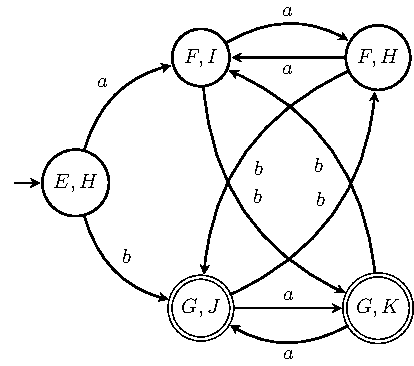
\includegraphics[width=0.5\linewidth]{A3xA4/A3xA4.pdf}%
        }
        \captionof*{figure}{Partie accessible de $\mathcal{A}_3 \times \mathcal{A}_4$}\label{fig:fig1}
        \end{minipage}

    \item \begin{minted}[breaklines]{ocaml}
    let produit aut1 aut2 = 
        let n1, delta1, f1 = aut1 in 
        let n2, delta2, f2 = aut2 in 
        let n = n1 * n2 in 
        let f = Array.make n false in
        let delta = Array.make n (0, 0) in
        let prod_etats n x1 x2 = (*fonction auxiliaire pour calculer delta d'un produit d'automates*)
        match x1, x2 with
        |(a, b), (c, d) -> n*a + c, n*b + d in
        for i = 0 to n1 - 1 do
            for j = 0 to n2 - 1 do
                begin
                if f1.(i) && f2.(j) then
                f.(n2 * i + j) <- true ;
                delta.(n2 * i + j) <- prod_etats n2 delta1.(i) delta2.(j) ;
                end
            done; done;
        partie_accessible (n, delta, f) ;;
    \end{minted}

    \item \label{itm:rec2} Soit $\mathcal{A}, \mathcal{A}'$ deux automates. \sloppy \newline
    Notons $\mathcal{P}(n)$ le prédicat : \og pour tout état $(q, q') \in Q_\mathcal{A} \times Q_{\mathcal{A}'}$ et pour tout mot $m$ de taille $n$, $\delta_{\mathcal{A} \times \mathcal{A}'}^*((q, q'), m) = (\delta_\mathcal{A}^*(q, m),\delta_{\mathcal{A}'}^*(q', m))$ \fg. Montrons par récurrence simple, que pour tout $n \in \bb{N}$, $\mathcal{P}(n)$. \\[2mm] 
    \underline{Initialisation} : Si $n = 0$, alors $m (= \varepsilon)$ est le mot vide, alors pour tout état $(q, q')$, $\delta_{\mathcal{A} \times \mathcal{A}'}^*((q, q'), \varepsilon) = (q, q')$ \newline 
    Or $\delta_\mathcal{A}^*(q, \varepsilon) = q$ et $\delta_{\mathcal{A}'}^*(q', \varepsilon) = q'$ donc $\delta_{\mathcal{A} \times \mathcal{A}'}^*((q, q'), \varepsilon) = (q, q') = (\delta_\mathcal{A}^*(q, \varepsilon), \delta_{\mathcal{A}'}^*(q', \varepsilon))$ \\[2mm]
    \underline{Hérédité} : Soit $n \in \bb{N}$, supposons $\mathcal{P}(n)$, montrons $\mathcal{P}(n) \Rightarrow \mathcal{P}(n + 1)$, \newline
    Soit $(q, q') \in Q_\mathcal{A} \times Q_{\mathcal{A}'}$ un état quelconque et $m$ un mot de taille $n + 1$, on peut alors noter $m = \sigma m_r$ où $m_r$ est un mot de taille $n$. Ainsi, \begin{eqnarray*}
        \delta_{\mathcal{A} \times \mathcal{A}'}^*((q, q'), m) & = & \delta_{\mathcal{A} \times \mathcal{A}'}^*(\delta_{\mathcal{A} \times \mathcal{A}'}((q, q'), \sigma), m_r) \text{ par définition de } \delta_{\mathcal{A} \times \mathcal{A}'}^* \\
        & = & \delta_{\mathcal{A} \times \mathcal{A}'}^*((\delta_\mathcal{A}(q, \sigma),\delta_{\mathcal{A}'}(q', \sigma)), m_r) \text{ par par définition de } \delta_{\mathcal{A} \times \mathcal{A}'} \\
        & = & (\delta_\mathcal{A}^*(\delta_\mathcal{A}(q, \sigma), m_r),\delta_{\mathcal{A}'}^*(\delta_{\mathcal{A}'}(q', \sigma), m_r)) \text{ d'après l'hypothèse de récurrence} \\
        & = & (\delta_\mathcal{A}^*(q, m),\delta_{\mathcal{A}'}^*(q',  m)) \text{ par définition de $\delta_\mathcal{A}^*$ et $\delta_{\mathcal{A}'}^*$}
    \end{eqnarray*}
    Donc $\forall n \in \bb{N}$, $\mathcal{P}(n)$ est vérifié. Ainsi, si $(q, q') \in Q_\mathcal{A} \times Q_{\mathcal{A}'}$ est un état accessible, alors il existe $m$ tel que $(q, q') = \delta_{\mathcal{A} \times \mathcal{A}'}^*((i_\mathcal{A}, i_{\mathcal{A}'}), m) = (\delta_\mathcal{A}^*(i_\mathcal{A}, m),\delta_{\mathcal{A}'}^*(i_\mathcal{A'}, m))$.\newline 
    Or comme $L(\mathcal{A}) = L(\mathcal{A}')$, $m \in L(\mathcal{A}) \Longleftrightarrow  m \in L(\mathcal{A'})$.  \fbox{D'où $q \in F_\mathcal{A} \Longleftrightarrow q' \in F_\mathcal{A'}$}.

    \item \label{itm:produit} Soit $\mathcal{A}, \mathcal{A}'$ deux automates accessibles qui acceptent le même langage. On considère $\mathcal{B}$ la partie accessible de $\mathcal{A} \times \mathcal{A'}$. \newline
    Montrons qu'il existe un morphisme d'automates $\varphi : \mathcal{B} -> \mathcal{A}$ : \newline
    Considérons $\varphi$ : $\begin{array}{ccc}
        \mathcal{B} & \to & \mathcal{A} \\
        (q, q') & \mapsto & q \\
        \end{array}$. \newline
    D'après la question \ref{itm:accessible}, comme $\mathcal{B}$ et $\mathcal{A}$ sont deux automates accessibles, il suffit de montrer que $\varphi$ vérifie $(2)$, $(3)$ et $(4)$ :
    \begin{itemize}
        \item Comme $i_\mathcal{B} = (i_\mathcal{A}, i_\mathcal{A'})$, on a directement $\varphi(i_\mathcal{B}) = i_\mathcal{A}$, ce qui montre que $\varphi$ vérifie $(2)$
        \item Si $(q, q') \in Q_\mathcal{B}$, alors pour tout $\sigma \in \{a, b \}$, on a à la fois $\varphi(q, q') = q$ par définition de $\varphi$ et $\varphi(\delta_\mathcal{B}((q, q'), \sigma)) = \varphi(\delta_\mathcal{A}(q, \sigma), \delta_\mathcal{A'}(q', \sigma)) = \delta_\mathcal{A}(q, \sigma)$. Donc $\varphi$ vérifie $(3)$.
        \item Enfin, soit $(q, q') \in Q_\mathcal{B}$ : 
            \begin{itemize}
                \item[($\Rightarrow$)] Si $(q, q') \in F_\mathcal{B}$, par définition de $\mathcal{B}$, $\varphi(q, q') = q \in F_\mathcal{A}$ ;
                \item[($\Leftarrow$)] Si $\varphi(q, q') = q \in F_\mathcal{A}$, alors d'après la question \ref{itm:rec2}, $q' \in F_\mathcal{A'}$, et donc $(q, q') \in F_\mathcal{B}$ ; 
            \end{itemize}
            Donc $\varphi$ vérifie également $(4)$
    \end{itemize}
    Ainsi, on démontre bien \fbox{l'existence d'un morphisme d'automates entre $\mathcal{B}$ et $\mathcal{A}$}. \newline
    \fbox{La symétrie du problème entre $\mathcal{A}$ et $\mathcal{A'}$} permet de conclure.
\end{enumerate}

\subsection{Diagramme d'automates}

\begin{enumerate}
    \setcounter{enumi}{21}

    \item Montrons que $\equiv$ définit bien une relation d'équivalence :
        \begin{itemize}
            \item Si $p \in Q_\mathcal{B}$ alors il existe une suite de longueur $0 + 1$ constituée du terme $ p = q_0 = p $ donc $p \equiv p $. Ainsi \fbox{$\equiv$ est réfléxive}.
            \item Soit $(p,q) \in Q_\mathcal{B}^2$ tel que $p \equiv q$, par définition, il existe une suite de longueur $k + 1 \in \bb{N^*}$ constituée des termes $p = q_0, q_1,..., q_k = q$, alors en considérant la suite constituée des termes $q = p_0, p_1, ..., p_{k - 1}, p_k = p$, où $ \forall \: 0 \leq j \leq k, p_j = q_{k - j}$ . Ainsi on a : \begin{multline*}
                \forall \: 0 \leq j < k, \; \varphi(p_{j + 1}) = \varphi(q_{\underbrace{k - j - 1}_{\in \llbracket 1 ; k \rrbracket}}) = \varphi(q_{k - j}) = \varphi(p_j) \\
                \text{ou   }  \psi(p_{j + 1}) = \psi(q_{\underbrace{k - j - 1}_{\in \llbracket 1 ; k \rrbracket}}) = \psi(q_{k - j}) = \psi(p_j)
            \end{multline*}
            Soit, $\forall \: 0 \leq j < k, \; \varphi(p_j) = \varphi(p_{j + 1}) \text{ ou } \psi(p_j) = \psi(p_{j + 1})$ \newline
            Ce qui montre $p \equiv q \implies q \equiv p$, et donc que \fbox{$\equiv$ est symétrique}.
            \item Soit $(p, q, r) \in Q_\mathcal{B}^3$ tel que $p \equiv q$ et $q \equiv r$, alors il existe deux suites, de taille respective $l + 1$ et $m + 1$ ($(\ell, m) \in \bb{N}^2$), constituées des termes $p = q_0, q_1, ... , q_\ell = q$ et $ q = r_0, r_1, ... , r_m = r$. \newline
            Alors en considérant la suite de taille $ k + 1 $ (où $ k = (\ell + m) \in \bb{N}$) constituée des termes \newline
            $p = q_0, q_1, ... , q_\ell = r_0, r_1, ... , r_m = r$, on a clairement :
            \begin{align*} \forall \: 0 \leq j < k, \; \varphi(p_j) = \varphi(p_{j + 1}) \text{ ou } \psi(p_j) = \psi(p_{j + 1}) \text{\footnotesize{(même lorsque $j = \ell$ puisque $\varphi(q_\ell) = \varphi(r_0) = \varphi(r_1)$)}} \end{align*}
            Donc $p \equiv q \land q \equiv r \implies p \equiv r$, ce qui conclut sur la \fbox{transitivité de $\equiv$}.
        \end{itemize}
        On a ainsi montré que \fbox{$\equiv$ est une relation d'équivalence}.

        \item \label{itm:transition} Soit $(p, q) \in Q_\mathcal{B}^2$ tel que $p \equiv q$. Soit $p = q_0, q_1, ..., q_k = q$ la suite associée à $\equiv$. \newline 
        Soit $\sigma \in \{a , b \}$, $j \in \llbracket 0;k \llbracket$. Si $\varphi(q_j) = \varphi(q_{j + 1})$, il découle :
        \begin{align*}
            \varphi(\delta_\mathcal{B}(q_j, \sigma)) &= \delta_\mathcal{A}(\varphi(q_j), \sigma) & \text{par propriété de morphisme de $\varphi$} \\
                                                    &= \delta_\mathcal{A}(\varphi(q_{j + 1}), \sigma) \\
                                                    &= \varphi(\delta_\mathcal{B}(q_{j + 1}, \sigma)) & \text{à nouveau par propriété de $\varphi$} \\
        \end{align*}
        Le résultat est clairement similaire avec $\psi$, si on suppose $\psi(q_j) = \psi(q_{j + 1})$. \newline
        Ainsi en définissant la suite $\Delta_0,\Delta_1, ..., \Delta_k$, avec $\forall j \in \llbracket 0 ; k \rrbracket, \; \Delta_j = \delta_\mathcal{B}(q_j, \sigma)$, alors
        \begin{equation*}
            \forall \: 0 \leq j < k, \; \varphi(\Delta_j) = \varphi(\Delta_{j + 1}) \text{ ou } \psi(\Delta_j) = \psi(\Delta_{j + 1}) \text{ (d'après ce que l'on vient de montrer).}
        \end{equation*}
        D'où le résultat : $\boxed{\delta_\mathcal{B}(p, \sigma) \equiv \delta_\mathcal{B}(q, \sigma)}$.

    \item \label{itm:final} Soit $(p, q) \in Q_\mathcal{B}^2$ tel que $p \equiv q$. Par symétrie de la relation $\equiv$, montrer que $ p \in F_\mathcal{B} \implies q \in F_\mathcal{B}$ suffira à montrer l'équivalence. \newline 
    Soit $p = q_0, q_1, ..., q_k = q$ la suite associée à $\equiv$. \newline
    Soit $j \in \llbracket 0;k \llbracket$. Si $\varphi(q_j) = \varphi(q_{j + 1})$, montrons que $q_j \in F_\mathcal{B} \implies q_{j + 1} \in F_\mathcal{B}$ : 
    \begin{equation*}
        q_j \in F_\mathcal{B} \implies \varphi(q_j) = \varphi(q_{j + 1}) \in F_\mathcal{A} \implies q_{j + 1} \in F_\mathcal{B} \;\; \text{(par propriété de morphisme de $\varphi$)}
    \end{equation*}
    Le résultat est clairement similaire avec $\psi$, si on suppose $\psi(q_j) = \psi(q_{j + 1})$. \newline
    Et donc, par une récurrence immédiate, $p \in F_\mathcal{B} \implies q \in F_\mathcal{B}$ et ainsi $\boxed{p \in F_\mathcal{B} \Longleftrightarrow q \in F_\mathcal{B}}$

    \item \label{itm:construC} Construisons un tel automate $\mathcal{C}$ :
        \begin{itemize}
            \item Comme imposé par l'énoncé : $ Q_\mathcal{C} = \{ S_0, S_1, ..., S_{l - 1} \}$ ;
            \item L'état initial $i_\mathcal{C}$ est $[i_\mathcal{B}]$ ;
            \item Comme montré à la question \ref{itm:transition}., si $\sigma \in \{a , b \}, \; (p, q) \in Q_\mathcal{B}^2$, alors $[p] = [q] \implies [\delta_\mathcal{B}(p, \sigma)] = [\delta_\mathcal{B}(q, \sigma)]$. \newline
                    On peut donc définir $\forall \sigma \in \{a, b\}, \: \forall [q] \in Q_\mathcal{C}, \; \delta_\mathcal{C}([q], \sigma) = [\delta_\mathcal{B}(q, \sigma)]$ ;
            \item De même, la question \ref{itm:final}. montre que si $[p] = [q]$ alors $p \in F_\mathcal{B} \Longleftrightarrow q \in F_\mathcal{B}$ donc on définit $F_\mathcal{C}$ ainsi : $F_\mathcal{C} = \{[q] \mid q \in F_\mathcal{B}\}$.
        \end{itemize}
        \fbox{$\text{On a ainsi construit }\mathcal{C} = \langle Q_\mathcal{C}, i_\mathcal{C}, \delta_\mathcal{C}, F_\mathcal{C} \rangle$}, montrons maintenant que $\eta$ est bien un morphisme d'automates de $\mathcal{B}$ vers $\mathcal{C}$. Comme $\mathcal{B}$ et $\mathcal{C}$ sont deux automates accessibles, il suffit de montrer que $\eta$ vérifie les conditions $(2), \: (3) \text{ et } (4)$ (question \ref{itm:accessible}.) :
        \begin{itemize}
            \item[(2)] Par définition de $i_\mathcal{C}$, on a clairement $\eta(i_\mathcal{B}) = [i_\mathcal{B}] = i_\mathcal{C}$ ;
            \item[(3)] Soit $q \in Q_\mathcal{B}, \: \sigma \in \{a , b \}$, Comme $\eta(q) = [q]$, on a clairement :
            \begin{equation*} \eta(\delta_\mathcal{B}(q, \sigma)) = [\delta_\mathcal{B}(q, \sigma)] = \delta_\mathcal{C}([q], \sigma) = \delta_\mathcal{C} (\eta(q), \sigma) \: ;
            \end{equation*}
            \item[(4)] Enfin, encore une fois d'après la définition de $\mathcal{C}$ : $\forall q \in Q_\mathcal{B}, \; q \in F_\mathcal{B} \Longleftrightarrow [q] = \eta(q) \in F_\mathcal{C}$ ;
        \end{itemize}
        \fbox{Donc $\eta$ est bien un morphisme d'automates de $\mathcal{B}$ vers $\mathcal{C}$}

    \item \label{itm:construMorphisme} Construisons un morphisme d'automates $\psi'$ tel que $\psi' \circ \psi = \eta$. \newline 
    Soit $q \in Q_\mathcal{A'}$, comme $\psi$ est surjective, il existe $p \in Q_\mathcal{B}$ tel que $q = \psi(p)$ et donc on définit : $\psi'(q) = [p]$. Supposons qu'il existe $p, p' \in  Q_\mathcal{B}$ tels que $q = \psi(p) = \psi(p')$, alors $p \equiv p'$ et donc $[p] = [p']$, ce qui montre bien que $\psi'(q')$ ne dépend pas de l'antécédent pas $\psi$ choisit, ce qui conclut bien sur la bonne définition de $\psi'$. \newline 
    Montrons maintenant que $\psi'$ est bien un morphisme d'automates. Comme $\mathcal{B}, \mathcal{A'}$ accessibles, il suffit de montrer que $\psi'$ vérifie $(2), \:(3)$ et $(4)$ (question \ref{itm:accessible}.) : 
    \begin{itemize}
        \item[(2)] Comme $i_\mathcal{A'} = \psi(i_\mathcal{B})$, $\psi'(i_\mathcal{A'}) = [i_\mathcal{B}] = i_\mathcal{C}$ ;

        \item[(3)] Soit $q \in \mathcal{A'}, \: \sigma \in \{a, b\}$, il existe $p \in Q_\mathcal{B}$ tel que $q = \psi(p)$. On a alors :
            \begin{align*}
                \delta_\mathcal{A'}(q, \sigma) &= \delta_\mathcal{A'}(\psi(p), \sigma)  & \\
                &= \psi(\delta_\mathcal{B}(p, \sigma)) & \text{par propriété de morphisme de $\psi$} \\
                \text{Donc } \psi'(\delta_\mathcal{A'}(q, \sigma)) &= \underbrace{\psi' \circ \psi}_{= \eta}(\delta_\mathcal{B}(p, \sigma)) & \\
                &= [\delta_\mathcal{B}(p, \sigma)] & \text{par définition de $\eta$ (cf question \ref{itm:construC}.)} \\
                &= \delta_\mathcal{C}([p], \sigma) & \text{par définition de $\delta_\mathcal{C}$ ((cf question \ref{itm:construC}.))} \\
                &= \delta_\mathcal{C}(\psi'(q), \sigma) & \text{car $\psi'(q) = [p]$ par construction}
            \end{align*}

        \item[(4)] Soit $q \in Q_\mathcal{A'}$, il existe $p \in Q_\mathcal{B}$ tel que $q = \psi(p)$ : 
            \begin{align*}
                q \in F_\mathcal{A'} & \Longleftrightarrow \psi(p) \in F_\mathcal{A'} & \\
                & \Longleftrightarrow p \in F_\mathcal{B} & \text{par propriété de morphisme de $\psi$} \\
                & \Longleftrightarrow [p] \in F_\mathcal{C} & \text{par définition de $F_\mathcal{C}$ (cf question \ref{itm:construC}.)} \\
                & \Longleftrightarrow \psi'(q) \in F_\mathcal{C} & \text{car $\psi'(q) = [p]$ par construction} 
            \end{align*}
    \end{itemize}
    Donc $\psi'$ ainsi construit est bien un morphisme d'automates de $\mathcal{A'}$ vers $\mathcal{C}$. En procédant de même avec $\varphi'$, en remplacant $\mathcal{A'}$ par $\mathcal{A}$, on \fbox{construit bien $\varphi'$ et $\psi'$ deux tels morphismes}.
    \item 
    \begin{minted}[breaklines]{ocaml}
    let maxi_positif arr = (*renvoie l'element maximum d'un tableau d'entiers positifs (et -1 si la liste est vide)*)
        if Array.length arr = 0 then -1 else
        let value = ref arr.(0) in 
        for i=1 to (Array.length arr) - 1 do
            value := max arr.(i) !value
        done; 
        !value ;; 
        
    let renomme arr =
        let size = Array.length arr in 
        let l = maxi_positif arr + 1 in (*entier l positif permettant de creer le dictionnaire (cf ci dessous)*)
        let index = Array.make l (-1) in (*semblant de dictionnaire qui a une valeur n associe une cle k (son indice dans le tableau renomme)*)
        let res = Array.make size 0 in (*tableau renomme*)
        let compteur = ref 0 in (*compteur permettant de garder en memoire la derniere cle associe a une valeur*)
        for i = 0 to size - 1 do
            begin
            if index.(arr.(i)) = -1 (*verifie que l'on a pas deja associe a la valeur n une cle*)
                then begin index.(arr.(i)) <- !compteur ;  (*on attribut a la valeur n une cle*)
                            incr compteur (*on incremente le compteur*)
                    end ;
            res.(i) <- index.(arr.(i)) (*on renomme le tableau*)
            end
        done;
        res ;;
    \end{minted}
    La fonction \verb|maxi_positif| à une complexité linéaire en $\ell$, et la fonction \verb|renomme| effectue une boucle fort comportant $n$ étapes (où $n$ est la taille du tableau donné en arguement). Les fonctions \verb|Array.make| sont aussi de complexité linéaire en $n$ pour \verb|res| et $\ell$ pour \verb|index|. \newline 
    Ainsi la fonction \cprotect\fbox{\verb|renomme| a une complexité en $O(\max(\ell, n))$}.

    \item 
    \begin{minted}[breaklines]{ocaml}
    let relation morph1 morph2 =
        let q_depart = Array.length morph1 in (*cardinal de l'automate de depart*)
        let q_arrive1 = maxi_positif morph1 + 1 in (*cardinal de l'automate image de phi*)
        let q_arrive2 = maxi_positif morph2 + 1 in (*cardinal de l'automate image de psi*)
        let voisins1 = Array.make q_arrive1 [] in (*voisins1.(q) = liste des antecedents de q par phi*)
        let voisins2 = Array.make q_arrive2 [] in (*voisins2.(q) = liste des antecedents de q par psi*)
        for i = 0 to (q_depart - 1) do (*on remplit les voisins*)
          voisins1.(morph1.(i)) <- i :: voisins1.(morph1.(i)) ;
          voisins2.(morph2.(i)) <- i :: voisins2.(morph2.(i))
        done;
        let morph_res = Array.make q_depart (-1) in (*initialisation de eta*)
        let rec aux e arr = function (*fonction auxiliaire qui pour tout i dans la liste va attribuer a arr.(i) la valeur e*)
          |[] -> ()
          |h::t -> morph_res.(h) <- e ; aux e arr t in
        for i = 0 to (q_depart - 1) do (*on remplit eta*)
          if morph_res.(i) = -1 then (*verifie si l'etat i ne s'est pas deja vu etre attribue une classe d'equivalence ...*)
            begin (*... si non, alors on initialise la classe d'equivalence (en lui donnant un numero quelconque (MAIS QUI N'A PAS ENCORE ETE DONNE))*)
              aux i morph_res voisins1.(morph1.(i)) ; (*on attribut cette classe d'equivalence aux voisins de q par phi*)
              aux i morph_res voisins2.(morph2.(i)) ; (*on attribut cette classe d'equivalence aux voisins de q par psi*)
            end
          else begin (*... si on a deja attribue une classe d'equivalence a cet etat, alors on l'attribut aux voisins de cet etat*)
            aux morph_res.(i) morph_res voisins1.(morph1.(i)) ;
            aux morph_res.(i) morph_res voisins2.(morph2.(i)) ;
          end
          done;
          renomme morph_res ;; (*on renomme les classes d'equivalence (notamment afin d'avoir morph_res.(0) = 0)*)
    \end{minted}
\end{enumerate}

\section{R\'eduction d'automates}

\subsection{Existence et unicit\'e}

\begin{enumerate}
    \setcounter{enumi}{28}
    
    \item \label{itm:construC2} D'après les questions \ref{itm:produit}. et \ref{itm:construC}, on peut \fbox{construire un automate $\mathcal{C}$} à partir de la partie accessible du produit d'automates $\mathcal{A} \times \mathcal{A'}$. \newline
    La question \ref{itm:construMorphisme}. assure \fbox{l'existence de deux morphismes $\varphi' : \mathcal{A} \to \mathcal{C}$ et  $\psi' : \mathcal{A'} \to \mathcal{C}$}.

    \item L'automate $\mathcal{A} \times \mathcal{A'}$ possède $2$ classes d'équivalence pour la relation $\equiv$ : $(E, H) \equiv (F, H) \equiv (F, I)$ et $(G, J) \equiv (G, K)$. On les note respectivement $S_0$ et $S_1$. \newline
    La représentation de $\mathcal{C}$ est donc : \newline
    \begin{minipage}[t]{\linewidth}
        \centering
        \captionof*{figure}{Automate $\mathcal{C}$}\label{fig:fig2}
        \adjustbox{valign=t}{%
            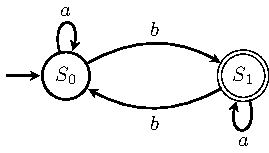
\includegraphics[width=0.3\linewidth]{C-30/C-30.pdf}%
        }
        \end{minipage}
    $\varphi' : \mathcal{A} \to \mathcal{C}$ est représentée par \begin{tabular}{|c|c|}
        \hline
        $q$ & $\varphi'(q)$ \\
        \hline
        $E$ & $S_0$ \\
        \hline
        $F$ & $S_0$ \\
        \hline
        $G$ & $S_1$ \\
        \hline
    \end{tabular}
    et $\psi'$ est représentée par \begin{tabular}{|c|c|}
        \hline
        $q$ & $\psi'(q)$ \\
        \hline
        $H$ & $S_0$ \\
        \hline
        $I$ & $S_0$ \\
        \hline
        $J$ & $S_1$ \\
        \hline
        $K$ & $S_1$ \\
        \hline
    \end{tabular}

    \item Soit $\mathcal{A}, \mathcal{A'} \in \mathfrak{R}_L$  (i.e $L = L(\mathcal{A}) = L(\mathcal{A'})$) tels que $|Q_\mathcal{A}| = |Q_\mathcal{A'}| = m_L$. \newline
    Par le même procédé qu'à la question \ref{itm:construC2}., on construit $\mathcal{C}$, $\varphi' : \mathcal{A} \to \mathcal{C}$ et $\psi' : \mathcal{A'} \to \mathcal{C}$. \newline
    Par surjectivité de $\varphi'$ et $\psi'$ : $|Q_\mathcal{C}| \leq m_L$. De plus l'existence de $\varphi'$ et $\psi'$ assure que $L(\mathcal{C}) = L(\mathcal{A}) = L(\mathcal{A'})$. Donc $\mathcal{C} \in \mathfrak{R}_L$, d'où $Q_\mathcal{C}| \geq m_L$ (par défintion de $m_L$). Donc $|Q_\mathcal{C}| = |Q_\mathcal{A}| = |Q_\mathcal{A'}|$. \newline
    Donc, d'après la question \ref{itm:isomorphisme}., $\varphi'$ et $\psi'$ sont des isomorphismes d'automates. \newline
    Toujours d'après la question \ref{itm:isomorphisme}, $\psi'^{-1}$ est aussi un isomorphisme d'automates, et donc comme composition d'isomorphismes : $\psi'^{-1} \circ \varphi'$ est un isomorphisme de $\mathcal{A}$ vers $\mathcal{A'}$ (cf question \ref{itm:composition}.). \newline
    \fbox{Donc $\mathcal{A}$ et $\mathcal{A'}$ sont nécessairement isomorphes}.

    \item Soit $\mathcal{A}, \mathcal{M}_L \in \mathfrak{R}_L$  (i.e $L = L(\mathcal{A}) = L(\mathcal{M}_L)$) tels que $|Q_{\mathcal{M}_L}| = m_L$. \newline
    Par le même procédé qu'à la question \ref{itm:construC2}., on construit $\mathcal{C}$, $\varphi' : \mathcal{A} \to \mathcal{C}$ et $\psi' : \mathcal{M}_L \to \mathcal{C}$. \newline
    Par surjectivité de $\psi'$ : $|Q_\mathcal{C}| \leq m_L$. De plus l'existence de $\varphi'$ et $\psi'$ assure que $L(\mathcal{C}) = L(\mathcal{A}) = L(\mathcal{A'})$. Donc $\mathcal{C} \in \mathfrak{R}_L$, d'où $Q_\mathcal{C}| \geq m_L$ (par défintion de $m_L$). Donc $|Q_\mathcal{C}| = |Q_{\mathcal{M}_L}|$. \newline
    Donc, d'après la question \ref{itm:isomorphisme}., $\psi'$ est un isomorphisme d'automates. \newline
    Toujours d'après la question \ref{itm:isomorphisme}, $\psi'^{-1}$ est aussi un isomorphisme d'automates, et donc comme composition de morphismes : $\varphi = \psi'^{-1} \circ \varphi'$ est un morphisme de $\mathcal{A}$ vers $\mathcal{M}_L$ (cf question \ref{itm:composition}.). \newline
    \fbox{Donc il existe bien un morphisme $\varphi : \mathcal{A} \to \mathcal{M}_L$}.
\end{enumerate}

\subsection{Construction d'un automate r\'eduit par fusion d'\'etats}

\begin{enumerate}
    \setcounter{enumi}{32}

    \item \begin{minipage}[t]{\linewidth}
        \centering
        \captionof*{figure}{Automate $\mathcal{A}_6^{O, P}$}\label{fig:fig3}
        \adjustbox{valign=t}{%
            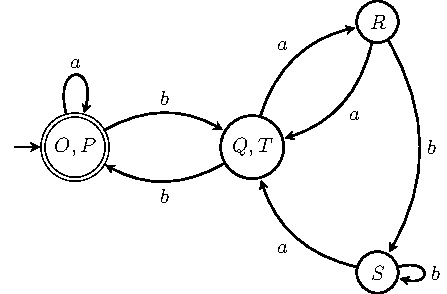
\includegraphics[width=0.5\linewidth]{A6OP/A6OP.pdf}%
        }
        \end{minipage}
    
    Afin de pouvoir créer un morphisme $\varphi$ de $\mathcal{A}_6$ vers $\mathcal{A}_6^{O, P}$, il faut aussi que l'on fussionne les états $Q$ et $T$ afin d'avoir les bonnes transitions par $b$. On peut alors représenter $\varphi$ par \begin{tabular}{|c|c|}
        \hline
        $q$ & $\psi'(q)$ \\
        \hline
        $O$ & $O, P$ \\
        \hline
        $P$ & $O, P$ \\
        \hline
        $Q$ & $Q, T$ \\
        \hline
        $R$ & $R$ \\
        \hline
        $S$ & $S$ \\
        \hline
        $T$ & $Q, T$ \\
        \hline
    \end{tabular}
    Ainsi, on a bien $\varphi(O) = \varphi(P)$ et $|Q_{\mathcal{A}_6^{O, P}}| < |Q_{\mathcal{A}_6}|$

    \item Les transitions des états $Q$ et $R$ selon $b$ dans $\mathcal{A}_6$ sont respectivment $O \in F_{\mathcal{A}_6}$ et $S \notin F_{\mathcal{A}_6}$. Ainsi par les propriétés $(3)$ et $(4)$ de morphisme de $\psi$, \fbox{il n'est pas possible d'avoir un tel $\mathcal{A}_6^{Q, R}$}.

    \item En partant de l'automate $\mathcal{A}_6^{O, P}$, on peut encore fusionner les états $R$ et $S$. \newline
    \fbox{On obtient alors un automate $\mathcal{M}_{L_6}$ à trois états qui reconnait le même langage que $\mathcal{A}_6$} : \newline
    \begin{minipage}[t]{\linewidth}
        \centering
        \adjustbox{valign=t}{%
            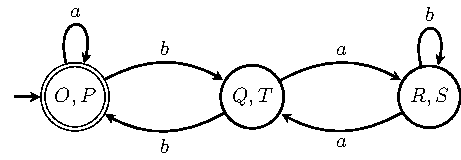
\includegraphics[width=0.5\linewidth]{Ml6/Ml6.pdf}%
        }
        \captionof*{figure}{Automate $\mathcal{M}_{L_6}$}\label{fig:fig4}
        \end{minipage}
    
    \item \label{itm:tabPredecesseurs} \begin{minted}[breaklines]{ocaml}
    let table_de_predecesseurs aut =
        let n, delta, f  = aut in 
        let tab = Array.make_matrix n n false in (*on initalise le tableau*)
        let rec aux p q = (*fonction auxiliaire qui visite tous les (p, q) pour un couple (p0, q0) donnee*)
        if not tab.(p).(q)  (*s'assure de ne visiter les sommets qu'une seule fois*)
        then begin
            tab.(p).(q) <- true ; 
            let succP_a, succP_b = delta.(p) in
            let succQ_a, succQ_b = delta.(q) in
            aux succP_a succQ_a ; (*début du parcours*)
            aux succP_b succQ_b ; (*suite du parcours (en profondeur)*)
            end
        in 
        for p = 0 to n - 1 do 
            for q = 0 to n - 1 do
                if (f.(p) && (not f.(q))) || ((not f.(p)) && f.(q)) (*pour tous les couples (p, q), on regarde si il respecte les conditions de l'enonce ...*)
                then aux p q (*... si oui, alors on le visite*)
            done;
        done;
        tab ;;
    \end{minted}

    \item On considère le graphe orienté $P'$ similaire à $P$ mais où l'orientation des arcs est inversée (i.e que pour tous $(p, q) \in Q \times Q$ et pour toute lettres $\sigma \in \{a , b \}$ les arcs vont de $(\delta(p, \sigma), \delta(q, \sigma))$ vers $(p, q)$). En faisant une fonction \verb|de_predecesseurs_bis|, simillaire à la fonction de la question \ref{itm:tabPredecesseurs}. mais pour le graphe $P'$, on aura alors \verb|tab.(p).(q) = false|  si et seulement si pour tout mot $m \in L(\mathcal{A})$, ($\delta_\mathcal{A}^*(p, m) \in F_\mathcal{A}$ et $\delta_\mathcal{A}^*(q, m) \in F_\mathcal{A}$) ou ($\delta_\mathcal{A}^*(p, m) \notin F_\mathcal{A}$ et $\delta_\mathcal{A}^*(q, m) \notin F_\mathcal{A}$). On dira que $p$ est en relation avec $q$ (et on notera cette relation $\star$). \newline
    Cette relation est clairement refléxive, symétrique et transitive, $\star$ est donc une relation d'equivalence. Ainsi pour réduire l'automate $\mathcal{A}$ on va déterminer les classes d'équivalence de la relation $\star$, et fusionner les états appartenant à chacune des classes. Pour ce faire, on determinera un morphisme $\varphi$ entre $\mathcal{A}$ et l'automate dont les états sont les classes d'équivalence de $\star$ (même procédé qu'à la question \ref{itm:construMorphisme}.), pour ensuite calculer l'image par $\varphi$ de $\mathcal{A}$ pour \fbox{obtenir $\mathcal{M}_L$}.

    \begin{minted}[breaklines]{ocaml}
    let table_de_predecesseurs_bis aut = 
        let n, delta, f = aut in
        let tab = Array.make_matrix n n false in
        let transi = Array.make_matrix n n [] in (*graphe P'*)
        for p = 0 to n - 1 do (*construction de P'*)
            for q = 0 to n - 1 do
                let succP_a, succP_b = delta.(p) in
                let succQ_a, succQ_b = delta.(q) in
                transi.(succP_a).(succQ_a) <- (p, q) :: transi.(succP_a).(succQ_a);
                transi.(succP_b).(succQ_b) <- (p, q) :: transi.(succP_b).(succQ_b);
            done;
        done;
        let rec aux p q = (*fonction auxiliaire qui parcours P' pour mettre a jour les relations "etoiles" entre les etats*)
            if not tab.(p).(q)
            then begin
                tab.(p).(q) <- true ; 
                List.iter (fun (i,j) -> aux i j) transi.(p).(q) ;
                end
        in
        for p = 0 to n - 1 do 
            for q = 0 to n - 1 do
                if (f.(p) && (not f.(q))) || ((not f.(p)) && f.(q))
                then aux p q
            done;
        done;
        tab ;;

    let etoile aut = (*meme procede que pour `relation` mais cette fois-ci on veut le morphisme et un etat quelconque dans chacune des classes*)
        let n, delta, f = aut in
        let pred = table_de_predecesseurs_bis aut in
        let classes_equiv = Array.make n (-1) in
        for p = 0 to n - 1 do
            if classes_equiv.(p) = -1
            then begin 
                classes_equiv.(p) <- p ;
                for q = 0 to n - 1 do 
                    if not pred.(p).(q) 
                    then classes_equiv.(q) <- p
                done;
                end
        done;
        let classes_equiv = renomme classes_equiv in
        let nb_classes = maxi_positif classes_equiv + 1 in
        let etats_classe = Array.make nb_classes (-1) in
        Array.iteri (fun i elem -> etats_classe.(elem) <- i) classes_equiv ;
        classes_equiv, etats_classe ;;

    let reduit aut = 
        let n, delta, f = aut in 
        let classes_equiv, etats_classe = etoile aut in
        let new_n = Array.length etats_classe in
        let new_delta = Array.make new_n (-1, -1) in 
        let new_f = Array.make new_n false in 
        for p = 0 to new_n - 1 do
            let succ_a, succ_b = delta.(etats_classe.(p)) in 
            new_delta.(p) <- classes_equiv.(succ_a), classes_equiv.(succ_b) ;
            new_f.(p) <- f.(etats_classe.(p))
        done ;
        (new_n, new_delta, new_f) ;;
    \end{minted}

    \textit{Exemple : en testant nos fonctions avec $\mathcal{A}_6$, on retrouve bien $\mathcal{M}_{L_6}$ :} \newline
    \begin{minted}[breaklines]{ocaml}
        INPUT :
        let a6 = let a6 = 6, [|(0, 2) ; (0, 5); (3, 1); (2, 4); (5, 4); (3, 0)|], [|true ; true ; false ; false ; false ; false|] in
        reduit a6 ;;

        OUTPUT : 
        - : int * (int * int) array * bool array =
        (3, [|(0, 1); (2, 0); (1, 2)|], [|true; false; false|])
    \end{minted}
\end{enumerate}
\end{document}